\documentclass[runningheads]{llncs}
\usepackage[hyphens]{url}
\usepackage{graphicx}
\usepackage{xcolor,colortbl}
\usepackage{mdframed}
\usepackage{multirow}
\usepackage{multicol}
\usepackage{comment}
\usepackage{lscape}
\usepackage{amsmath}
\usepackage{scrextend}
\usepackage[utf8]{inputenc}
\usepackage[T1]{fontenc}
\usepackage[inline]{enumitem}
\usepackage{multido}
%\usepackage{pstricks}
\usepackage{tikz}
\usetikzlibrary{intersections}
\usepackage{pifont}% http://ctan.org/pkg/pifont
\newcommand{\cmark}{\ding{51}}%
\newcommand{\xmark}{\ding{55}}%
% Used for displaying a sample figure. If possible, figure files should
% be included in EPS format.
%
% If you use the hyperref package, please uncomment the following line
% to display URLs in blue roman font according to Springer's eBook style:

\mdfdefinestyle{RQFrame}{
 outerlinewidth=0pt,
 skipabove=0pt,
 skipbelow=0pt,
 innertopmargin=6pt,
 innerbottommargin=0pt,
 linewidth=0pt,
 topline=false,
 rightline=false,
 leftline=false,
 innerrightmargin=4pt,
 innerleftmargin=4pt}

\newcounter{RQCounter}
\newcommand{\RQ}[2]{
\refstepcounter{RQCounter} \label{#1}
\begin{mdframed}[style=RQFrame]\noindent
    \textbf{RQ}$_{\arabic{RQCounter}}$.~\emph{#2}
\end{mdframed}
}
\newcommand{\hr}[1]{\textbf{RQ}$_{\ref{#1}}$}
\definecolor{Gray}{gray}{0.9}
\newcommand{\mysubsec}[1]{\smallskip \emph{\textbf{#1.}}}

\usepackage{amssymb}% http://ctan.org/pkg/amssymb
\usepackage{pifont}% http://ctan.org/pkg/pifont


\usepackage{hyperref}
\renewcommand\UrlFont{\color{blue}\rmfamily}

\begin{document}
%
\title{Security Risk Estimation and Management in Autonomous Driving Vehicles}
%
\titlerunning{Security Risk Estimation and Management in Autonomous Driving Vehicles}
% If the paper title is too long for the running head, you can set
% an abbreviated paper title here
%
\author{Abasi-amefon O. Affia \and Raimundas Matulevi\v{c}ius \and Rando T\o{}nisson}
\institute{University of Tartu, Tartu, Estonia\\
\email{\{amefon.affia, rma\}@ut.ee} \\
}

%
%\authorrunning{}
\authorrunning{Affia et al.}
% First names are abbreviated in the running head.
% If there are more than two authors, 'et al.' is used.
%
%
\maketitle              % typeset the header of the contribution
%

\begin{abstract}
Security risk management is an important activity in engineering autonomous vehicles (AV). However, developing a secure intelligent information system (IIS) typically poses challenges to the  organizations business goals and budget constraints that require addressing only a subset of the threats to the IISs developed.
For autonomous driving service providers, it is necessary to estimate risks exposures of threats, the severity of the threat impacts and how they could be mitigated. This process of security risk estimation and mitigation allow system stakeholders to manage the security risks within their systems. %Unfortunately, an accepted standard to carry out security risk management, specifically for autonomous vehicles, is not presented in the reviewed literature.
In this paper, we explore how to protect AV systems against the security risks and focusing on the security risks of its autonomous components. To target the problem we employ the security risk management (ISSRM) and operationally critical threat, asset and vulnerability evaluation (OCTAVE \textit{allegro})  methods to define and estimate the AV protected asset, risk and risk treatment means.
%
Our findings can be helpful to the AV engineers and security analysis to support the rationale for the decisions about the AV security investment. 

\keywords{Autonomous vehicles \and self-driving cars \and security risk management \and ISSRM \and OCTAVE}
\end{abstract}



\section{Introduction}
Securing the rising amount of internet of things (IoT) systems and applications, gathering, managing and presenting data from distributed sources and through its perception, network, and application layers~\cite{AffiaEtAl2019}, is an increasingly vital task. 
%
Computing systems can centralize and manipulate data from other IoT layers comprising of intelligent information processing nodes (i.e., complex gateways, servers and subsystems).
In today’s highly automated landscape, the trend towards information aggregation from multiple asset sources is on the rise and applies specifically in autonomous systems.
%
Autonomous driving vehicles are highly complex information sensing, processing and actuating systems, harmonizing diverse information models~\cite{banerjee2017aggregation}. As such, pulling information from multiple assets within the system context for purposes of analysis, diagnostics, navigation etc., is of high importance to an autonomous driving vehicle.
%
Autonomous driving vehicles as intelligent information systems have taken advantage of its ability to collect, perceive, generate and disseminate information between vehicular and infrastructure systems. These activities improve knowledge to act autonomously, providing its required services of mobility, safety, and comfort to the human components of its ecosystem.  
%
Autonomous driving generates sensitive information about customers, including information about where and when the passenger is using the car. Also, it collects data about the environment, different objects like obstacles and traffic signs, which are essential for the self-driving. Therefore it is necessary to secure these data and information against the malicious use. There exist studies~\cite{Bailey2018,ElRewiniEtAl2020} on security risk assessment and security engineering in the AV systems, however these studies \textit{do not consider the AV as an IIS}. 
In this study, we analyse \textit{how autonomous vehicles can be protected against the security risks}. We split the main research question into three sub-questions. 

\begin{itemize}
\item \textbf{RQ1}: What are the protected AV assets?
\item \textbf{RQ2}: What are security risks and their estimated impact on AVs? 
\item \textbf{RQ3}: What are security countermeasures to mitigate the security risks in AV based on their estimated impact?
\end{itemize}

All three sub-questions are incrementally considered by performing three subsequent research steps: (\textit{i}) literature/background study, (\textit{ii}) case analysis, and (\textit{iii}) discussion of our analysis. The background study (see Sect.~\ref{sec:appr}) resulted in defining the scope of the work, security risk management methods proposed for AVs and \textit{initial} AV system and business assets, security risks and countermeasures to mitigate security risks, found in literature. 

The background also provided a basis for combining the domain model for information system security risk management (ISSRM)~\cite{DuboisEtAl2010}, with the operationally critical threat, asset and vulnerability evaluation (OCTAVE \textit{allegro})~\cite{CaralliEtAl2007} to explore the security risks to AV. After the background study, we conduct a case analysis (see Sect.~\ref{sec:case}) where we apply the elicited information in the case of the autonomous components of the actual AV in the laboratory settings. Again the analysis is guided by the ISSRM domain model where we also apply the OCTAVE method to estimate the risk impact and the cost of the identified countermeasures. We validate the results (see Sect.~\ref{sec:disc}) and provide our findings. We also compare our findings and method to risk estimation and management to related work (see Sect.~\ref{sec:related}) in literature, showing the need for an approach that strongly considers AV as IISs. Our findings can be helpful to the AV engineers and security analysts to support the rationale for decisions about the AV security investments.


\section{Background and Related Work}
\label{sec:appr}
\subsection{Scope of work}
%The following outlines important definitions in this work and thus forming the scope of our work.

We form our study around important definitions and taxonomies outlining the scope of our work. 
%within the scope of security in autonomous driving vehicles. 
%\textbf{Security Engineering.}
%Security vs Safety
Ensuring security in AVs form the backbone of our work. 
``\textit{Security engineering} is concerned with lowering the risk of intentional unauthorized harm to valuable assets to a level acceptable to the system's stakeholders by preventing and reacting to malicious threats and security risks''~\cite{firesmith2007engineering}. 
Hence, security in the context of this paper deals specifically with intentional unauthorized threats and risks that explicitly pose harm to the AV system assets. Security engineering is thus different from safety engineering (which is not the focus of this work) dealing with unintentional risk, leading to accidental consequences in the AV physical environment.
%
%\textbf{Automotive technology.}
%Vehicular automotive technology is the practical application of knowledge about on-road, self-propelled and commonly wheeled vehicles, that do not operate on rails. Advances in the automotive industry constantly drives towards research interest in automation and autonomous driving~\cite{pettersson2017design}. As, automated and AVs are only a subset of vehicular automotive technology, in this study we will not generalise to a literature study on vehicular automobiles but focus on its advancing subsets. 

%\textbf{Automation in Vehicles.}
%Automated vehicles
We also understand that the realisation of AVs is made possible by \textit{automation} -- the use of electronic or mechanical devices to augment or replace human activity applied to operating a road vehicle. In this study, we focus on highly automated components of vehicular automotives. The SAE J3016~\cite{vehicle2016j3061} standard defines six levels of motor vehicle driving automation systems, ranging from no driving automation at all (level 0) to full driving automation (level 5). %
%For automation, vehicles that are equipped with a multitude of sensors interacting to form a driving automation system capable of delivering multiple driving automation features performing at different levels (0 - 5). Thus, the level of automation exhibited at any instance and by any vehicle is determined by the automation features engaged for that vehicle.
%
%
\textit{Autonomy} in vehicles is achieved where there are high levels of automation. Following the SAE J3016~\cite{vehicle2016j3061} standard, an AV is one in which achieves level 4 and level 5 vehicular automation. Level 4 vehicular automation refers to semi-AVs able to autonomously, without any human/driver intervention, perform all driving functions under \textbf{\textit{certain conditions}} (e.g. on a specific type of road or or at certain times). Level 5 vehicular automation on the other hand refers to fully AVs able to autonomously perform all driving functions under \textbf{\textit{all conditions}}.
%
Although our study on security risk estimation and management can apply to vehicles with lower levels of automation, in this paper we focus only on vehicles that have achieved \textbf{\textit{autonomy}}, which are the semi-autonomous and fully AVs.  


\subsection{Security Risk Management Methods in AV}
There exist different standards for securing vehicles at different levels of automation. These standards include ISO 26262 standard~\cite{palin2011iso}, SAE J3061 standard~\cite{vehicle2016j3061}, ISO/SAE 21434~\cite{SAECybersecurity}, NIST SP 800 53r4~\cite{joint2013nist}. 
These standards define general guidelines or best practices for information security and security risk management activities in AV. However, a good security risk management method follows well known standards, and presenting a process for security risk estimation and management.

There exists also different methods aimed at security risk management, relevant for use in AVs. These methods have been recommended by relevant standards~\cite{vehicle2016j3061} and they include the EVITA method~\cite{evita2011safety}, ETSI Threat, Vulnerability, and implementation Risk Analysis (TVRA) standard~\cite{etsi2011182}, Operationally Critical Threat, Asset, and Vulnerability Evaluation (OCTAVE)~\cite{CaralliEtAl2007}, HEAVENS security model~\cite{olovsson2018healing}, and the Security-aware hazard and risk analysis method (SAHARA)~\cite{macher2015sahara}. 
Though the aforementioned standards and methods can act as the guidelines when considering AV security, there is still a lack of consistency in the approaches for identifying vulnerabilities, threats/attacks, risk assessment and estimation, as well as risk treatment. Consequently, we did not find a standard or method in literature proposed to be applicable to AV security %(covering its vulnerabilities, threats/attacks, risk assessment and estimation, as well as risk treatment) 
given its complex capabilities and overlap across multiple information domains and able to provide enough risk-based information for business decisions.

%Octave was designed to securely orchestrate IoT data, protecting IoT application data from end-to-end. 
%There is a need for methods that analyse the complex information sensing, processing and actuating systems, as well as the diverse information models in AVs. 
The OCTAVE method~\cite{CaralliEtAl2007} is one method that assesses information security risks for supporting decisions about security investment. The method includes pre-prepared templates to support and document risk management activities, and guide data collection for probability and security risk impact estimation. These risk estimation activities help to reason about the security countermeasures to treat security risks. Although OCTAVE provides a strong method for security risk estimation, it is not as strong in its risk analysis process. In this study, we introduce the ISSRM domain model~\cite{DuboisEtAl2010} to guide through explicit security risk identification by supporting elicitation of assets, attack methods, vulnerabilities, threats, risks, and countermeasures to mitigate identified risks.
%combine OCTAVE with 
Originally developed for information systems risk management, the ISSRM domain model is also applicable in the AV systems as these systems are basically used to gather, manipulate, interpret and \textit{disseminate} information for the stakeholders. Combination of the OCTAVE and ISSRM methods complements and strengthens the analysis (\textit{i}) with the ISSRM guidance for the security risk identification and definition and (\textit{ii}) with the OCTAVE templates for security risk impact and countermeasure estimation. 

\subsection{Related Work}\label{sec:related}

Related work exists, analysing in part or in whole, on the topic of managing security risks related to autonomous driving vehicles.
%
%Attack experiments on sensors used in AV are explained in~\cite{YanEtAl2016,PetitEtAl2015}. Maple~\textit{et al.}~\cite{MapleEtAl2019} provided AV reference architecture and attack surface analysis. Elsewhere in~\cite{ScalasEtAl2019} Scalas and Giacinto describe the potential AV vulnerabilities and some approaches to fix. 
In Table~\ref{tab:relatedwork} we aggregated the outcome on the literature study to AVs that focus on AV security including its potential security threats, risk impact, risk estimations and suggested countermeasures.

From our analysis, Dominic~\textit{et al}, and Parkinson~\textit{ et al}~\cite{dominic2016risk,parkinson2017cyber} covered the security risk estimation and management scope focusing on security engineering and covering potential security threats, risk impact, risk estimations and suggested countermeasures in AVs. However, there are limited details or documentation in~\cite{dominic2016risk,parkinson2017cyber} on the impact of the security threat on AV system assets. %Also there are limited details on the risk estimation and the context of autonomy in~\cite{PetitEtAl2014}.
Other related works~\cite{chattopadhyay2020autonomous,cui2019review,malik2020analysis,AffiaEtAl2019,dibaei2020attacks,de2020driverless,lima2016towards,kong2018security} covered the security risk management scope, some focusing on both safety and security engineering and covering potential security threats, risk impact and suggested countermeasures in AVs. However, these papers no not discuss estimations needed for business decisions.
%
%
%
Interestingly, in Boudguiga~\textit{et al}.,~\cite{boudguiga2015race} proposed a method, named RACE, combining TVRA and EVITA to propose a unique risk computation method. However, the method did not apply cost of countermeasure to the risk estimations creating a challenge for business decisions.
%

Our paper provides a security focused risk estimation and management analysis, covering the security threats, its impacts, proposed countermeasures and risk estimations based on the mentioned security metrics. We provide a detailed documentation of these concepts showing appropriate rationale for making business decisions on securing AVs.


%\begin{landscape}
\begin{table}[htp!]
\vspace{-15pt}
    \centering{
    \label{tab:relatedwork}
    \caption{Comparison with literature related to security risk estimation and management in AVs.}
    \resizebox{\textwidth}{!}{%
    \begin{tabular}{|p{0.33\linewidth}|p{0.08\linewidth}|p{0.08\linewidth}|p{0.1\linewidth}|p{0.13\linewidth}|p{0.15\linewidth}|p{0.1\linewidth}|}
    \hline
        Related Work & \multicolumn{4}{c|}{Risk management} &  \multirow{2}{*}{Autonomous} &  \multirow{2}{*}{Security} \\  \cline{2-5}
         & Threat & Impact & Solution & Estimation & Focus & Focus \\ \hline
         
        Chattopadhyay \textit{et al}~\cite{chattopadhyay2020autonomous} & \ding{51} & LD & \ding{51} &  \ding{55} & \ding{51} & \ding{51} \\ \hline
        Parkinson \textit{ et al}~\cite{parkinson2017cyber} & \ding{51} & LD & \ding{51} & \ding{51} & \ding{51} & \ding{51} \\ \hline
        %Petit and Shladover~\cite{PetitEtAl2014} & \ding{51} & LD & \ding{51} & \ding{51} & \ding{51} &  \ding{51} \\ \hline
        %Cui \textit{et al}~\cite{cui2019collaborative} & \ding{51} & LD & \ding{51} & \ding{55} & \ding{51} &  SS \\ \hline
        Malik and Sun~\cite{malik2020analysis} & \ding{51} & LD & \ding{55} & \ding{55} & \ding{51} &  \ding{51} \\ \hline
        Boudguiga~\textit{et al}~\cite{boudguiga2015race} & \ding{51} & \ding{51} & \ding{55} & \ding{51} & LD &  SS \\ \hline
        Cui~\textit{et al}~\cite{cui2019review} & \ding{51} & LD & \ding{51} &  \ding{55} & \ding{51} & SS \\ \hline
        Affia~\textit{et al}~\cite{AffiaEtAl2019} & \ding{51} & \ding{51} & \ding{51} &  \ding{55} & LD & \ding{51} \\ \hline
        Dibaei~\textit{et al}~\cite{dibaei2020attacks} & \ding{51} & LD & \ding{51} & \ding{55} & \ding{51} & \ding{51} \\ \hline
        De La Torre~\textit{et al}~\cite{de2020driverless} & \ding{51} & LD & \ding{51} & \ding{55} &   \ding{51} & \ding{51} \\ \hline
        Lima~\textit{et al}~\cite{lima2016towards} & \ding{51} & LD & \ding{51} & \ding{55} & \ding{51} & SS \\ \hline
        Dominic~\textit{et al}.~\cite{dominic2016risk} & \ding{51} & \ding{51} & \ding{51} & LD & LD & \ding{51} \\ \hline
        Kong~\textit{et al}~\cite{kong2018security} & \ding{51} & \ding{51} & \ding{55} & \ding{55} & \ding{51} & \ding{51} \\ \hline
        This Paper &  \ding{51} & \ding{51} & \ding{51} &  \ding{51} & \ding{51} & \ding{51} \\ \hline
        \multicolumn{7}{c}{{\raggedright \ding{51} - Detailed Discussion; LD - Limited Discussion; \ding{55} - No Discussion; \par}} \\
         \multicolumn{7}{c}{{\raggedright SS - Discusses security and safety. \par }}
    \end{tabular} }
 \vspace{-15pt}  } 
\end{table}
%\end{landscape}


\subsection{AV system analysis}

To secure gathered, manipulated and disseminated data, and its asset source within an autonomous driving vehicle, we study AV assets found in literature.

\textbf{System Assets}. Security modelling is based on knowing the system assets.
Following~\cite{AffiaEtAl2019}, the AV system can be decomposed to perception, network and application layers as illustrated in \hyperref[fig:AssetModel]{Fig.~\ref{fig:AssetModel}}. \textit{Perception layer} includes 
the system components responsible for collecting data. In AV, those are devices for sensing, positioning, and seeing; such as radars, LiDAR, global positioning systems (GPS), cameras~\cite{YanEtAl2016,ThingEtAL2016,PetitEtAl2015} and other. \textit{Network layer} is used to transfer the data between the perception and application layers. The transfer can be wireless or wired; the vehicle could also use its own in-vehicle networks (e.g., controller area network (CAN) and local area network (LAN))~\cite{ThingEtAL2016}. CAN is used to exchange data between different components in the vehicle; LAN -- to deliver data from sensors to the application layer. The AVs are also connected to the Internet. The \textit{application layer} is responsible for connecting to end-users. It consists of computers, servers, data storage and humans if needed. The application layer uses the collected data to calculate routes and based on these calculation to control the car. The calculations are done using a computing unit (i.e., industry-oriented computers)~\cite{ThingEtAL2016}. The calculation results can then be converted into commands, the actuation module will use those to perform autonomous functions. The layer also includes electronic control units (ECU) to control the electronics in the car.

\begin{figure}[h!]
  \vspace{-15pt}
  \centering
  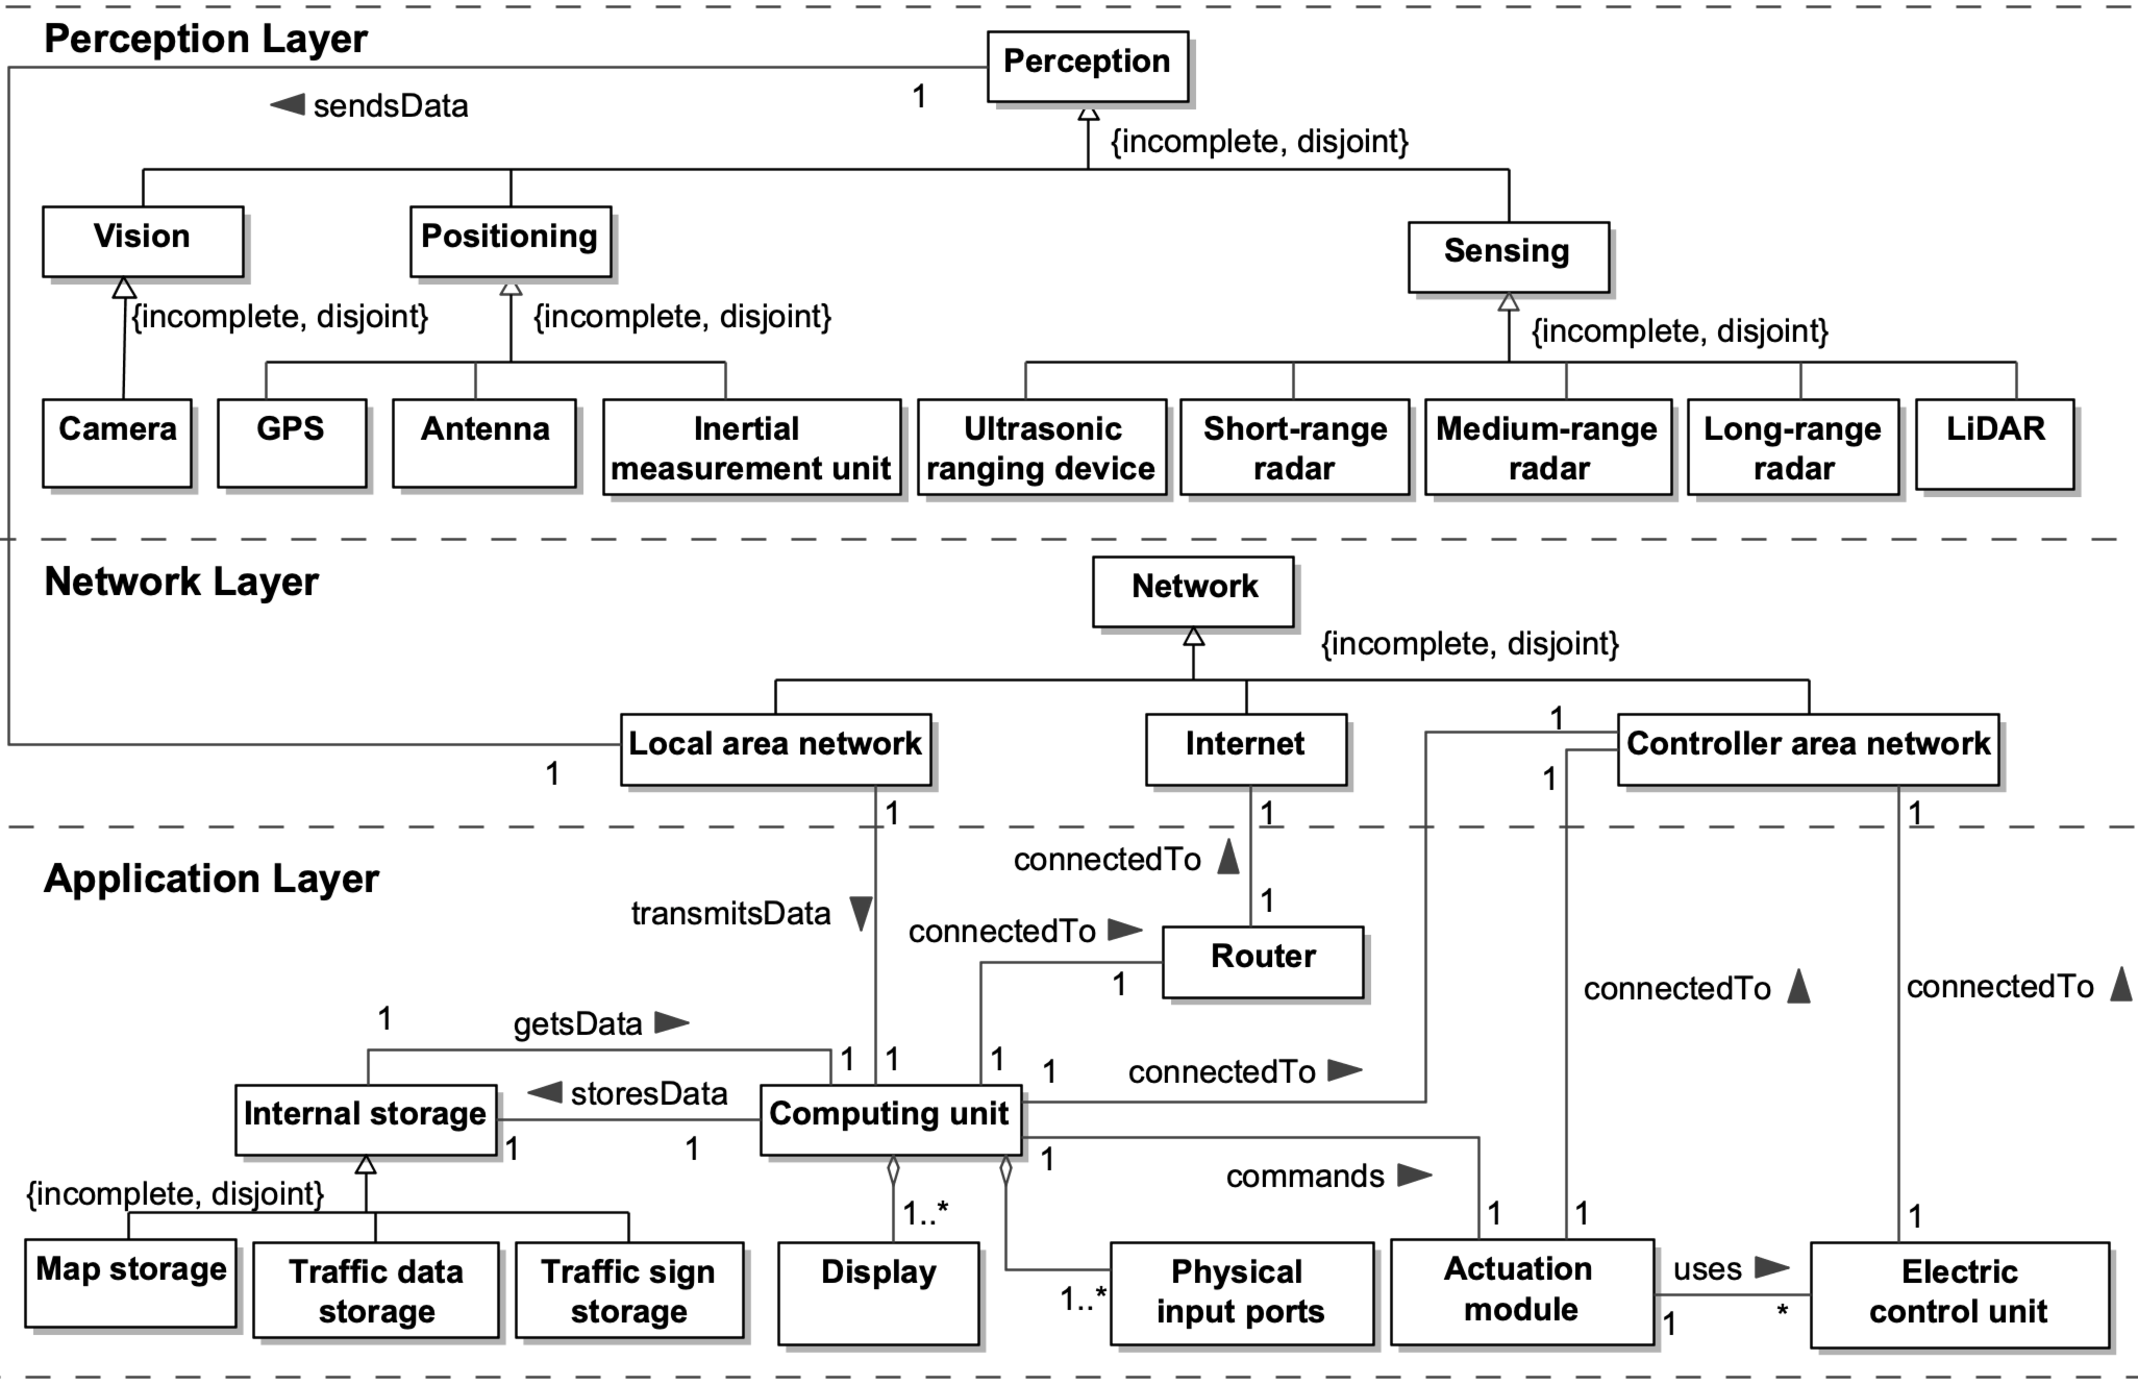
\includegraphics[width=0.9\linewidth]{AVasset}
  \caption{Literature study: AV system assets} 
  \label{fig:AssetModel}
  \vspace{-15pt}
\end{figure}
%\begin{figure}[h]
%   \centering
%   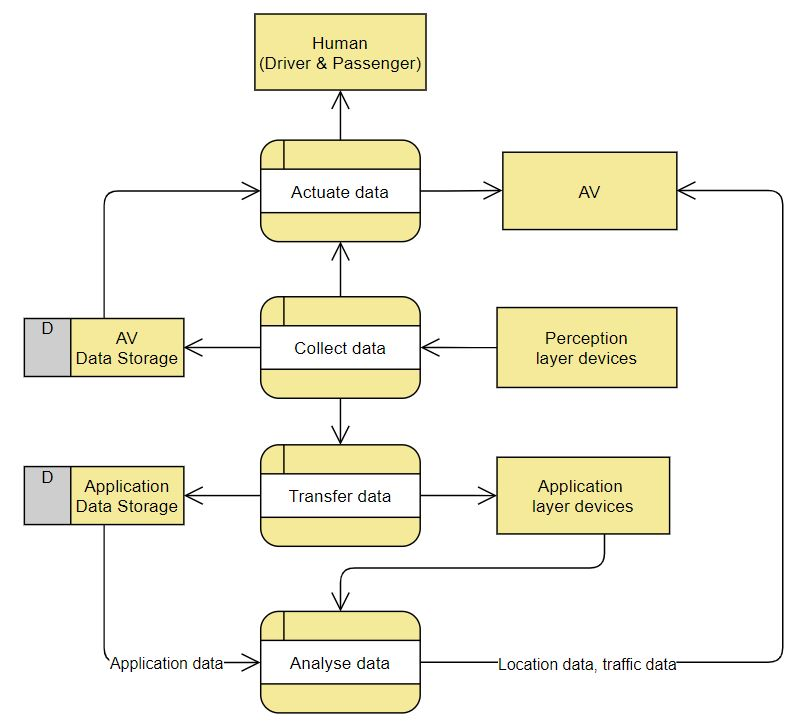
\includegraphics[width=0.7\linewidth]{AV-DFD.JPG}
%    \caption{Simple Data flow diagram of AV} 
%    \label{Fig:AVarchi}
%\end{figure}
\textbf{Business assets} are defined as data and information what are valuable in the system. Security need is estimated using the security criteria (i.e., confidentiality, integrity and availability) on the business assets. At the \textit{perception layer}, business assets (such as \textit{video data, image data, vehicle location data, vehicle travel data, working vehicle data, ultrasonic sensors data, surrounding environment data, radar data, inertial measurements data, measurement data} and others) are data collected by the system assets of this layer. After collection, the \textit{communication data} is transmitted through the \textit{network}. But communication data can also include messages and data exchanged between components of the \textit{application layer}. 
%
In the \textit{application layer}, the data is processed by the computing unit, which also fuses them with the data from internal storage.  
Depending on the computation purpose, the business assets at the application level include \textit{map data, traffic data, traffic sign data, computing data, actuation’ commands data, fused data, ECU’s data, decision-maker, driving planner, autonomous driving data} and similar.

\textbf{Security Threats and Risks} specifically crucial for the AV system will be the focus of our analysis. We did not include risks describing regular cars, meaning that we only take into account security risks that affect the AV sensors, communication between the AV components, or the other components to achieve autonomous driving.
%
In literature, we have identified security risks (see \hyperref[tab:risks]{Table~\ref{tab:risks}}, columns 1-3). Eleven risks (R1-R9, R16 %and R24
) are identified at the perception layer, seven (R10-R11, R19-R23) -- at the application layer, and four (R12-R15) at the network layer. R17 can be found at all layers, and R18 is identified at the network and application layers. Details of security risks are discussed within our case study in Sect.~\ref{sec:case} and could also be found in~\cite{Rando2020}. We do not consider the risks in Table~\ref{tab:risks} as exhaustive but aim to raise awareness of the security risks that can be found in AVs.

\begin{table}[h!]
\caption{Literature study: Security risks and countermeasures}
\label{tab:risks}
 \vspace{-10pt}  
\resizebox{\textwidth}{!}{%
\begin{tabular}{|l|l|l|l|l|}
\hline
\textbf{Risk ID} & \textbf{Literature} & \textbf{Risk name} & \textbf{Countermeasure} & \textbf{Literature} \\ \hline
R1  & \textbf{[1, 2, 3]} & Jamming ultrasonic sensors & Noise detection and rejection; Multiple sensors for redundancy check 
%
& \textbf{[1]} \\ \hline
R2  &~\cite{YanEtAl2016} ~\cite{YanEtAl2016}~\cite{ThingEtAL2016} & Spoofing ultrasound sensors & Noise detection and rejection; Multiple sensors for redundancy check &~\cite{YanEtAl2016} \\ \hline
R3  &~\cite{YanEtAl2016} ~\cite{YanEtAl2016}~\cite{PetitEtAl2014} & Acoustic quieting on ultrasound sensors & Multiple sensors for redundancy check &~\cite{YanEtAl2016} \\ \hline

R4  &~\cite{YanEtAl2016}~\cite{MapleEtAl2019}~\cite{ThingEtAL2016}~\cite{PetitEtAl2014} & Jamming radar & Noise detection and rejection; Multiple sensors for redundancy check &~\cite{YanEtAl2016} \\ \hline
R5  &~\cite{YanEtAl2016}~\cite{MapleEtAl2019}~\cite{ThingEtAL2016}~\cite{PetitEtAl2014} & Spoofing radar & Noise detection and rejection; Multiple sensors for redundancy check &~\cite{YanEtAl2016} \\ \hline
R6  &~\cite{YanEtAl2016}~\cite{MapleEtAl2019}~\cite{PetitEtAl2015} & Blinding cameras & Overlapping image output (multiple cameras); Filter to remove harmful light &~\cite{YanEtAl2016}~\cite{PetitEtAl2015} \\ \hline
R7  & ~\cite{PetitEtAl2015} & Confusing car controls using camera inputs & Overlapping image output (multiple cameras); Filter to remove harmful light &~\cite{YanEtAl2016}~\cite{PetitEtAl2015} \\ \hline
R8  &~\cite{MapleEtAl2019} ~\cite{PetitEtAl2015} & Relay attack on LiDAR & Multiple LiDAR inputs; Random probing; Shorten pulse period &~\cite{YanEtAl2016}~\cite{PetitEtAl2015} \\ \hline

R9  & ~\cite{MapleEtAl2019}~\cite{ThingEtAL2016}~\cite{PetitEtAl2015} & Spoofing LiDAR & Multiple LiDAR inputs; Random probing; Shorten pulse period &~\cite{YanEtAl2016}~\cite{PetitEtAl2015}  \\ \hline
R10 &~\cite{ThingEtAL2016} & Code modification & Device authentication; Anti-Malware; Isolation & ~\cite{ThingEtAL2016}~\cite{ScalasEtAl2019}  \\ \hline
R11 &~\cite{ThingEtAL2016} & Code injection & Device authentication; Anti-Malware; Isolation &~\cite{ThingEtAL2016}~\cite{ScalasEtAl2019} \\ \hline
R12 &~\cite{ThingEtAL2016}~\cite{ScalasEtAl2019} & Packet sniffing & Encryption; Device and user authentication &~\cite{ThingEtAL2016}~\cite{ScalasEtAl2019} \\ \hline
R13 &~\cite{MapleEtAl2019}~\cite{ThingEtAL2016} ~\cite{ScalasEtAl2019} & Packet fuzzing & Encryption; Device and user authentication &~\cite{ThingEtAL2016}~\cite{ScalasEtAl2019} \\ \hline
R14 & ~\cite{PetitEtAl2014} & Inject CAN messages & Encryption; Device and user authentication &~\cite{ThingEtAL2016}~\cite{ScalasEtAl2019}  \\ \hline
R15 &~\cite{MapleEtAl2019}~\cite{PetitEtAl2014} & Eavesdropping CAN messages & Encryption; Device and user authentication &~\cite{ThingEtAL2016}~\cite{ScalasEtAl2019}\\ \hline
R16 & ~\cite{MapleEtAl2019,PetitEtAl2014,parkinson2017cyber} & GPS: Jamming and spoofing  & Nullification, Monitoring signals and identification nodes & ~\cite{ThingEtAL2016,o2013real} \\ \hline
R17 &~\cite{PetitEtAl2014}& EMP attack & Isolation &~\cite{ThingEtAL2016}~\cite{ScalasEtAl2019} \\ \hline
R18 &~\cite{PetitEtAl2014} & Malware injection & Firewall; Anti-Malware; Isolation & ~\cite{ThingEtAL2016} \\ \hline
R19 & ~\cite{MapleEtAl2019}~\cite{PetitEtAl2014} & Manipulate map data & User authentication; Device authentication; Isolation &~\cite{ThingEtAL2016}~\cite{ScalasEtAl2019} \\ \hline
R20 &~\cite{MapleEtAl2019} & Extract map data & User authentication; Device authentication; Isolation &~\cite{ThingEtAL2016}~\cite{ScalasEtAl2019} \\ \hline
R21 &~\cite{MapleEtAl2019} & Delete map data & User authentication; Device authentication; Isolation &\cite{ThingEtAL2016}~\cite{ScalasEtAl2019}  \\ \hline
R22 &\cite{MapleEtAl2019} & Disable actuation module & Isolation; Access control &~\cite{ThingEtAL2016}~\cite{ScalasEtAl2019} \\ \hline
R23 &~\cite{MapleEtAl2019} & Induce bad analysis & Isolation; Access control; Input validation &~\cite{ThingEtAL2016}~\cite{ScalasEtAl2019}\\ \hline
%R24 & ~\cite{MapleEtAl2019,PetitEtAl2014,parkinson2017cyber,tippenhauer2011requirements} & GPS spoofing & --  &~\cite{o2013real} \\ \hline
\end{tabular}%
}
 \vspace{-15pt}  
\end{table}

\textbf{Countermeasures}. Countermeasures identified in literature are presented in \hyperref[tab:risks]{Table~\ref{tab:risks} (see columns 4 and 5)}. Countermeasures at the perception layer are discussed in~\cite{YanEtAl2016,PetitEtAl2015}. In~\cite{YanEtAl2016} Yan \textit{et al.} discuss noise detection and rejection. A small amount of noise is normal for the sensors to pick up, but detecting sudden big outburst of that can indicate some malicious activity; therefore, sensors should have noise detection controls. Another security control is multiple input sources for redundancy check~\cite{YanEtAl2016}. Multiple sensors could reduce the impact of the risks as targeting all sensors at the same time requires more attack means and expertise. To make redundancy check harder to work around, Yan~\textit{et al.}~\cite{YanEtAl2016} recommended to add randomness to the control parameters and built-in attack detection system. Thing and Wu~\cite{ThingEtAL2016} discuss that cameras could be protected using light filters to detect and filter the harmful light sources (e.g., lasers). To secure LiDAR, one recommends random probing. To protect against attacks described in ~\cite{PetitEtAl2015} one recommends adding randomness to the rotation speed. However, some LiDAR devices require constant rotating speed so the random probing cannot be used. In such cases, shortening the pulse period could make it harder for an attacker to send the pulse at the right time. To avoid GPS jamming, nullification is suggested in ~\cite{ThingEtAL2016} as jamming only requires that enough radio noise on the GPS frequency to block authentic signals from the GPS receiver. Nullification refers to the usage of security and electronic capabilities of the devices to invalidate or neutralise the attack. For GPS spoofing, simple mechanisms such as monitoring identification codes, satellite signals, and the use of time intervals can help detect spoofing attempts. However, it has been revealed in literature that nothing short of a military-grade implementation can effectively prevent GPS spoofing~\cite{ThingEtAL2016,PetitEtAl2014}. 

The most recommended countermeasures at the network layer are encryption, special devices and user authentication techniques~\cite{ThingEtAL2016}~\cite{ScalasEtAl2019}. Knowing where the data came from could help from being harmed by the attacker (who could send the malicious code or malware). For the application layer risks, countermeasures are derived from ~\cite{ThingEtAL2016}~\cite{ScalasEtAl2019}. Authors advise using the anti-malware software and firewalls in/on the computing unit. User authentication could help to detect who sends and what data is sent. Authentication would also reduce the chance for outsiders to gain access to any of the components. In addition to authentication, access control methods should be implemented. Knowing who and when have tried to gain access to some component help stop the spread of malicious software. There should also be ways to isolate the affected components, to avoid giving access to attackers, and to prevent the spread of malware.


\section{Case Analysis}
\label{sec:case}

 A case analysis was carried out in the laboratory environment where we considered the the Lexus RX450h AV, designed to support AutonomouStuff~\footnote{\url{https://autonomoustuff.com/product/lexus-rx-450h}}. %\cite{AS}. 
 
\textbf{System Assets}. The car has a pre-built system to support driving by wire, meaning the car is controllable using a game controller. That system is the basis for autonomous driving as it allows controlling the car using electrical inputs. The game controller can be replaced with a computer giving the inputs instead of a human. 

\textit{LiDAR} consists of a laser, scanner and GPS receiver. It is used to map out of surrounding vehicles and objects while driving. The data then is used to make driving decisions. In our case VLP32C~\footnote{\url{https://velodynelidar.com/products/ultra- puck/}} has been used. It has a 360-degree horizontal and 40-degree vertical field of view and has a working range of 200 meters. In AV \textit{cameras} are used to detect and identify traffic signs, lights, pedestrians and other vehicles (and predicts their movements) using machine learning algorithms. In the analysed car  different cameras were used: Mako cameras~\footnote{\url{https://www.alliedvision.com/en/products/cameras/detail/Mako20G/G- 319/}} %\cite{AlliedVision} 
to gather visual data and SF332X-10X cameras~\footnote{\url{http://sekolab.com/products/camera/}} %\cite{Sekonix} 
to capture a 120-degree view. \textit{Radars} are used to get speed and range data of the vehicles around the radar for braking and lane changing.
The range of the radar can vary from short to long. In our case, Delphi ESR 2.5 24V~\footnote{\url{https://autonomoustuff.com/product/delphi-esr-2-5-24v/}} %\cite{AutonomousStuff} 
radar with capabilities of medium to long-range is used.
\textit{Global positioning system} (GPS) use the satellites to get accurate data of the location and time. The car was equipped with Novatel GPS PwrPak7~\footnote{\label{note1}\url{https://www.novatel.com/products/gnss-receivers/enclosures/pwrpak7}}, and paired with an \textit{inertial measurement unit} (IMU) -- IMU-IGM-S1/STIM30~\footnote{\label{note2}\url{https://www.novatel.com/products/span-gnss-inertial-systems/span-imus/span-mems-imus/imu-igm-s1/}}, which uses gyro and accelerometer to collect the 3D navigation data. In addition, Novatel GPS antennas are used to get better tracking performance. \textit{Computing unit} is used to handle a large amount of information. In the analysed case Spectra industrial computer~\footnote{\url{https://www.neousys- tech.com/en/product/application/edge-ai-gpu-computing/nuvo-6108gc-gpu-computing}} (with a GTX2080 GPU, GIGe Ethernet card and Kvaser 4x channel card) is installed. In AV \textit{actuation module} is responsible for steering, accelerating, braking and other driving operations, which are controlled by the electronic control units (ECU). In the considered case the platform actuation and control module (PACMod)~\footnote{\url{ https://autonomoustuff.com/product/pacmod/}} is used. 

The analysed AV is equipped with components that make the testing, driving and development process more convenient. The wAP router~\footnote{\url{https://help.mikrotik.com/docs/display/UM/wAP+ac+kit-series}} is installed to connect the car to the Internet. The Kvaser USB to CAN hub is used to connect the computers to the CAN network. In addition, a standard USB hub is added to connect different convenience components like a keyboard and mouse. Multiple screens are installed in the car to monitor the driving process.

\textbf{Business assets}. \hyperref[tab:Business Assets]{Table~\ref{tab:Business Assets}} illustrates the business assets and how they are supported by the components of the analysed AV at the three architecture layers. Note, all vehicle components support the \textit{autonomous driving} as a service.

\begin{table}[h!]
\caption{Case analysis: Business and system assets}
\label{tab:Business Assets}
 \vspace{-10pt} 
\resizebox{\textwidth}{!}{%
\begin{tabular}{|l|l|l|l|}
\hline
\textbf{Layer} &
  \textbf{Business   asset} &
  \textbf{Description} &
  \textbf{Associated   system assets} \\ \hline
\multirow{9}{*}{Perception} &
  Video data &
  Video from surrounding environment &
  Mako G, Sekonix cameras \\ \cline{2-4} 
 &
  Picture data &
  Pictures from surrounding environment &
  Mako G, Sekonix cameras \\ \cline{2-4} 
 &
  Vehicle location data &
  Current location of the vehicle &
  PwrPak7 GPS, IGM-S1 IMU \\ \cline{2-4} 
 &
  Vehicle travel data &
  Routes used with the time &
  PwrPak7 GPS, IGM-S1 IMU \\ \cline{2-4} 
 &
  Working vehicle data &
  Vehicle speed, direction etc. &
  PwrPak7 GPS, IGM-S1 IMU \\ \cline{2-4} 
 &
  Ultrasonic sensors data &
  Ultrasonic data about surroundings &
  Ultrasonic sensors \\ \cline{2-4} 
 &
  Radar data &
  Data from radar &
  Delphi ESR 24V \\ \cline{2-4} 
 &
  Surrounding environment data &
  \begin{tabular}[c]{@{}l@{}}Data about the surrounding \\ environment and objects\end{tabular} &
  \begin{tabular}[c]{@{}l@{}}VLP32 LiDAR, Delphi ESR \\ 24V, Ultrasonic sensors\end{tabular} \\ \cline{2-4} 
 &
  Inertial measurements &
  Vehicle speed, angle, location &
  IGM-S1 IMU \\ \hline
Network &
  Communication data &
  \begin{tabular}[c]{@{}l@{}}Data and messages exchanged by \\ different components\end{tabular} &
  Network \\ \hline
\multirow{7}{*}{Application} &
  Map data &
  Map used for autonomous driving &
  Map storage \\ \cline{2-4} 
 &
  Fused data &
  Combined data from perception layer &
  \begin{tabular}[c]{@{}l@{}}Perception layer, network, \\ Spectra computer\end{tabular} \\ \cline{2-4} 
 &
  Computing data &
  Results from analysing the fused data &
  Spectra computer \\ \cline{2-4} 
 &
  Actuation commands data &
  \begin{tabular}[c]{@{}l@{}}Commands generated to be sent to \\ actuation module\end{tabular} &
  \begin{tabular}[c]{@{}l@{}}Spectra computer, PACMod \\ v3.0, ECU\end{tabular} \\ \cline{2-4} 
 &
  Decision maker &
  Software for making driving decisions &
  Spectra computer \\ \cline{2-4} 
 &
  Driving planner &
  Software for planning out the route used &
  Spectra computer \\ \cline{2-4} 
 &
  System software &
  All software used for autonomous driving &
  Spectra computer \\ \hline
All &
  Autonomous driving &
  Overall process of vehicle self-driving &
  All components \\ \hline
\end{tabular}%
}
 \vspace{-10pt}  
\end{table}
% end of Business assets

\textbf{Security risks}. The architecture of the car is presented in \hyperref[fig:AssetRiskModel]{Fig.~\ref{fig:AssetRiskModel}}, it is an instance of model from our literature study (see \hyperref[fig:AssetModel]{Fig.~\ref{fig:AssetModel}}). The figure also illustrates how risks are associated. 
\hyperref[tab:risk-example]{Table~\ref{tab:risk-example}} shows an example of one risk -- R6.
Here, \textit{an attacker with some expertise and tools to send malicious optical inputs}; this way he disturbs the cameras with malicious optical outputs. This threat targets the  \textit{cameras}(system assets), because \textit{cameras are vulnerable to blinding attacks}. If the event happens, it negates the \textit{integrity of video and image data}. This leads to the unreliable data and could provoke wrong decisions when car is driving/steering. In~\cite{Rando2020} all security risks are explicitly defined using the domain model~\cite{DuboisEtAl2010} as illustrated in \hyperref[tab:risk-example]{Table~\ref{tab:risk-example}}.


\begin{figure}[h!]
  \centering
    \vspace{-10pt} 
  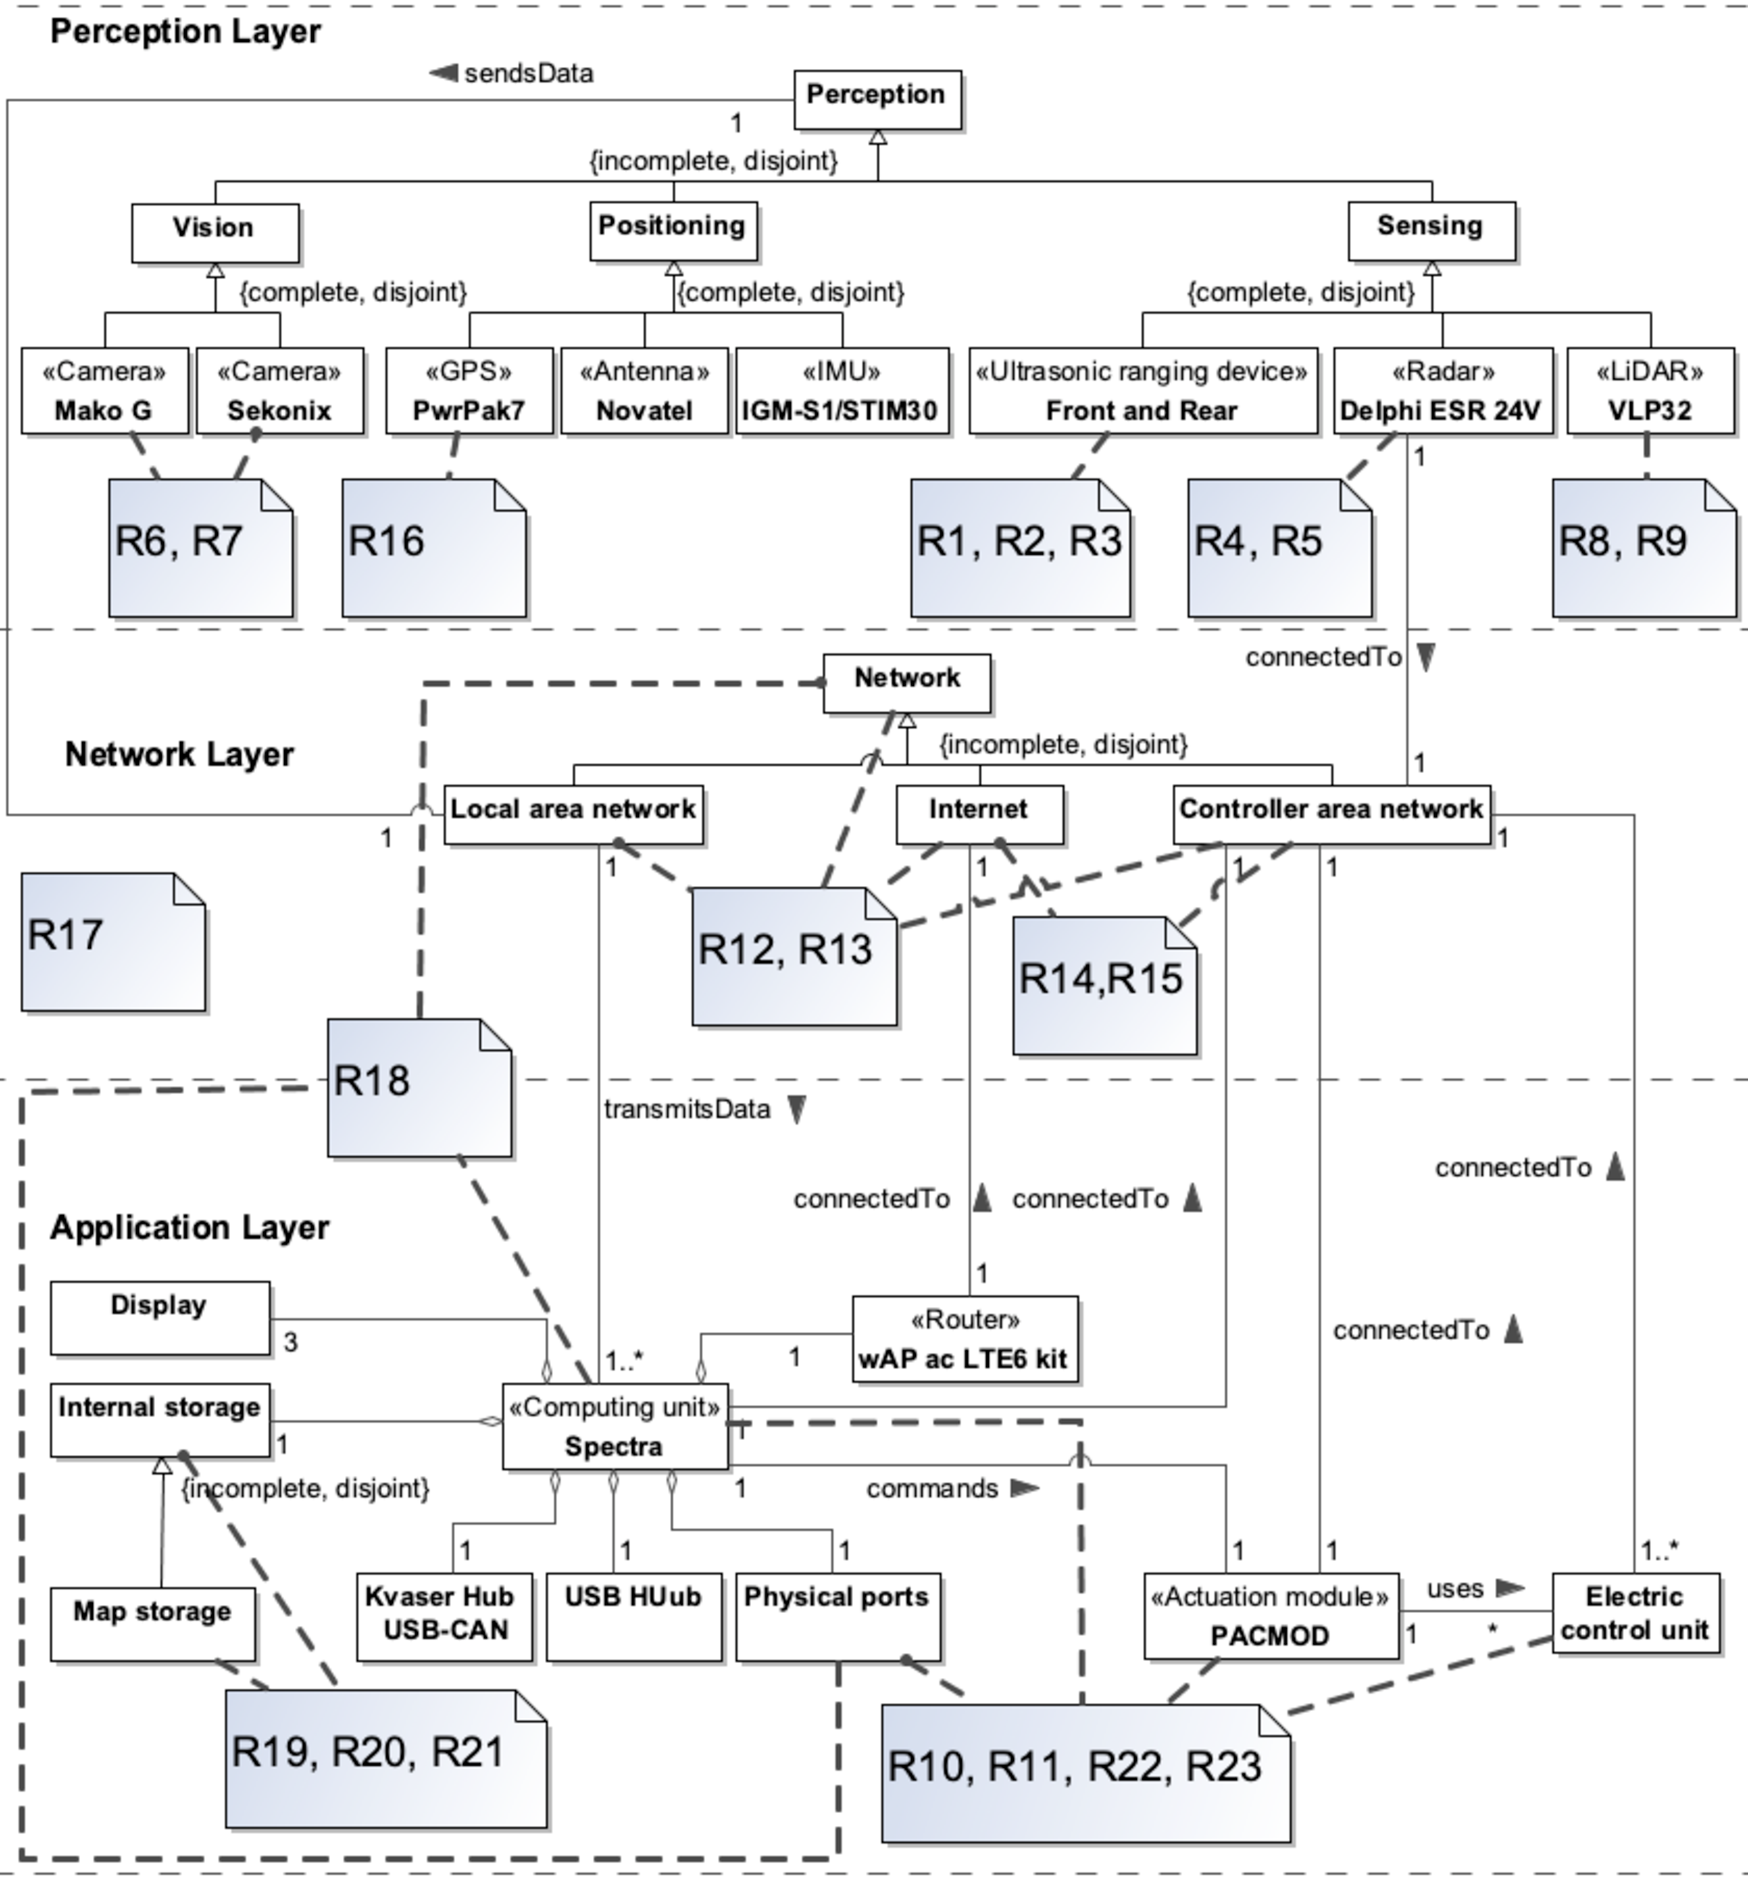
\includegraphics[width=0.8\linewidth]{AVassetsCase}
  \caption{Case analysis: AV assets and associated security risks} 
  \label{fig:AssetRiskModel}
   \vspace{-15pt}  
\end{figure}

\begin{table}[h!]
\caption{Security risk definition using ISSRM domain model (R6: Blinding cameras)}
\label{tab:risk-example}
 \vspace{-5pt} 
\resizebox{\textwidth}{!}{%
\begin{tabular}{|l|l|}
\hline
\textbf{Business asset} & Video and image data  \\ \hline
\textbf{Security criteria} & Integrity of video and image data \\ \hline
\textbf{System asset} & Cameras \\ \hline
\textbf{Risk ID} & R6 Blinding cameras\\ \hline
\textbf{Risk} &
  \begin{tabular}[c]{@{}l@{}}An attacker uses their tools to send  \\ malicious optical data to the camera causing unwanted blindness, possible \\ hardware damage and loss of integrity of video and image data.\end{tabular} \\ \hline
\textbf{Impact} &
\begin{tabular}[c]{@{}l@{}}Loss of integrity of video and image data;  \\ provoke wrong decision when steering the vehicle.\end{tabular} \\ \hline
\textbf{Vulnerability} & Cameras are vulnerable to blinding attacks. \\ \hline
\textbf{Threat} &
  \begin{tabular}[c]{@{}l@{}}An attacker uses their knowledge and malicious optical \\ emitters to send and blind cameras causing unwanted blindness \\ on the cameras and possibly permanently damage the camera sensors.\end{tabular} \\ \hline
\textbf{Threat agent} &
  \begin{tabular}[c]{@{}l@{}}An attacker with some previous experience and  \\ tools to send malicious optical inputs (laser etc.).\end{tabular} \\ \hline
\textbf{Attack method} & 
  \begin{tabular}[c]{@{}l@{}}An attacker can disturb the cameras with malicious \\ optical outputs to blind the cameras.\end{tabular} \\ \hline
\end{tabular}%
}
 \vspace{-15pt} 
\end{table}

The impact of each security risk is estimated using the OCTAVE approach. The business value of an asset is estimated based on the value it provides to the system. The main concern is to explain what happens if the data is lost or modified. The \textit{low} score is assigned if system can stay operational without this asset; \textit{medium} - if the system can continue, but there exist some performance issues; and \textit{high} - if the system becomes not operational. Similarly the threat {likelihood} is estimated as \textit{low} if the needed means to perform the attack method are specific and their cost is high, the required knowledge to perform the attack method is high, and possibility to carry on the attack method require much time. The likelihood is estimated as \textit{high} if it is easy to obtain the means for execute the attack method, not much knowledge and preparation is required. An example of the risk estimation is given in \hyperref[tab:octave-example]{Table~\ref{tab:octave-example}}. Following this approach to total risk score for the R6 is 48. The summary of the risk estimation is illustrated in \hyperref[tab:riskEstimation]{Table~\ref{tab:riskEstimation} (see column 4)}, which indicates that \textit{highly} estimated risks are 
R6 and R16; \textit{lowly} -- R3, R14, R17, R19, R20, and R21.

% octave example table
\begin{table}[h!]
\caption{Risk estimation using OCTAVE (R6: Blinding cameras)}
\label{tab:octave-example}
\resizebox{\textwidth}{!}{%
\begin{tabular}{lllll|l|l|l|l|l|l|l|l|l|l|l|l|l|l|}
\hline
\multicolumn{2}{|l|}{\textbf{Allegro – Worksheet 10}} &
  \multicolumn{17}{l|}{\textbf{R6 – Blinding attack on cameras}} \\ \hline
\multicolumn{1}{|l|}{\multirow{9}{*}{\rotatebox[origin=c]{90}{\textbf{Threat}}}} &
  \multicolumn{1}{l|}{\textbf{Business   Asset}} &
  \multicolumn{17}{l|}{video and image data} \\ \cline{2-19} 
\multicolumn{1}{|l|}{} &
  \multicolumn{1}{l|}{\textbf{Business Asset’s Value}} &
  \multicolumn{17}{l|}{Medium – Car can continue driving but can’t recognize signs and traffic lights.} \\ \cline{2-19} 
\multicolumn{1}{|l|}{} &
  \multicolumn{1}{l|}{\textbf{Area of Concern}} &
  \multicolumn{17}{l|}{\begin{tabular}[c]{@{}l@{}}An attacker uses their tools to send malicious optical data to the camera causing\\ unwanted blindness, possible hardware damage and loss of integrity of\\ video and image data.\end{tabular}} \\ \cline{2-19} 
\multicolumn{1}{|l|}{} &
  \multicolumn{1}{l|}{\begin{tabular}[c]{@{}l@{}}\textbf{Actor}   \\ Who would exploit the area of \\ concern or threat?\end{tabular}} &
  \multicolumn{17}{l|}{\begin{tabular}[c]{@{}l@{}}An attacker with some previous experience and tools to send malicious \\ optical inputs (laser etc.).\end{tabular}} \\ \cline{2-19} 
\multicolumn{1}{|l|}{} &
  \multicolumn{1}{l|}{\begin{tabular}[c]{@{}l@{}}\textbf{Means}  \\ How would the actor do it?  \\ What would they do?\end{tabular}} &
  \multicolumn{17}{l|}{\begin{tabular}[c]{@{}l@{}}An attacker uses their knowledge and malicious optical emitters to send \\ and blind cameras causing unwanted blindness on the cameras and possibly \\ permanently damage the camera sensors.\end{tabular}} \\ \cline{2-19} 
\multicolumn{1}{|l|}{} &
  \multicolumn{1}{l|}{\begin{tabular}[c]{@{}l@{}}\textbf{Motive} \\ What is the actor’s reason for doing it?\end{tabular}} &
  \multicolumn{17}{l|}{Wants to see the car crash and make the company lose reputation.} \\ \cline{2-19} 
\multicolumn{1}{|l|}{} &
  \multicolumn{1}{l|}{\begin{tabular}[c]{@{}l@{}}\textbf{Outcome} (choose one)  \\ What would be the resulting effect be?\end{tabular}} &
  \multicolumn{3}{l|}{Disclosure:} &  \hspace{1cm} 
   &
  \multicolumn{2}{l|}{Destruction:} &
  \multicolumn{3}{l|}{ \hspace{1cm} } &
  \multicolumn{3}{l|}{Modification:} &
  \multicolumn{3}{l|}{ \hspace{1cm} } &
  Interruption: & \hspace{5mm} 
  x \hspace{5mm} \\ \cline{2-19} 
\multicolumn{1}{|l|}{} &
  \multicolumn{1}{l|}{\begin{tabular}[c]{@{}l@{}}\textbf{Security Requirements}  \\ How would the information asset’s  \\ security requirements be breached?\end{tabular}} &
  \multicolumn{17}{l|}{Cameras are vulnerable to   blinding attacks.} \\ \cline{2-19} 
\multicolumn{1}{|l|}{} &
  \multicolumn{1}{l|}{\textbf{Likelihood} (choose one)} &
  \multicolumn{2}{l|}{High:} &
  \multicolumn{3}{l|}{  \hspace{1cm} x  \hspace{2cm} } &
  \multicolumn{3}{l|}{Medium:} &
  \multicolumn{3}{l|}{ \hspace{2cm} } &
  \multicolumn{2}{l|}{Low:} &
  \multicolumn{4}{l|}{ \hspace{1cm} } \\ \hline
\multicolumn{3}{|l|}{\begin{tabular}[c]{@{}l@{}}\textbf{Consequences}  \\ What are the consequences to the organization as a result of the risk?\end{tabular}} &
  \multicolumn{16}{l|}{\begin{tabular}[c]{@{}l@{}}\textbf{Severity} \\ How severe are the consequences to the \\ organization or asset owner by  \\  impact area?  \\ *3 for highest priority, 2 for medium,  \\  1 for lowest\end{tabular}} \\ \hline
\multicolumn{3}{|l|}{Blinding attack will cause some blind spots on the image recorded by the cameras.} &
  \multicolumn{6}{l|}{\textbf{Impact area}} &
  \multicolumn{3}{l|}{\textbf{Priority*}} &
  \multicolumn{4}{l|}{\textbf{Impact}} &
  \multicolumn{3}{l|}{\textbf{Score}} \\ \cline{4-19} 
\multicolumn{3}{|l|}{Blind spots can cause not   detecting objects and possible accidents because of that.} &
  \multicolumn{6}{l|}{Confidentiality} &
  \multicolumn{3}{l|}{1} &
  \multicolumn{4}{l|}{Low} &
  \multicolumn{3}{l|}{1} \\ \cline{4-19} 
\multicolumn{3}{|l|}{\begin{tabular}[c]{@{}l@{}}Not having the sensor available without any mitigations will cause the system to not\\ see the outside, possibly other sensors can cover.\end{tabular}} &
  \multicolumn{6}{l|}{Availability} &
  \multicolumn{3}{l|}{3} &
  \multicolumn{4}{l|}{High} &
  \multicolumn{3}{l|}{9} \\ \cline{4-19} 
\multicolumn{3}{|l|}{Using lasers to carry out   the attack can permanently damage the camera’s lens.} &
  \multicolumn{6}{l|}{Integrity} &
  \multicolumn{3}{l|}{2} &
  \multicolumn{4}{l|}{High} &
  \multicolumn{3}{l|}{6} \\ \hline
\multicolumn{5}{l}{} &
  \multicolumn{11}{l|}{Relative   risk score:} &
  \multicolumn{3}{l|}{16} \\ \cline{6-19} 
\multicolumn{5}{l}{} &
  \multicolumn{11}{l|}{Total   Risk Score (Rel x likelihood):} &
  \multicolumn{3}{l|}{48} \\ \cline{6-19} 
\end{tabular}%
}
 \vspace{-15pt}  
\end{table}
% octave example end


% risks
\begin{table}
\caption{Security Risks and scores for Bolt prototype.}
\label{tab:riskEstimation}
\scriptsize
\resizebox{\textwidth}{!}{%
\begin{tabular}{|l|l|l|l|}
\hline
\textbf{Risk ID} & \textbf{Risk name} & \textbf{Associated system assets} & \textbf{Risk score} \\ \hline
R1  & Jamming ultrasonic sensors & Ultrasonic ranging devices & 32  \\ \hline
R2  & Spoofing ultrasound sensors & Ultrasonic ranging devices & 32 \\ \hline
R3  & Acoustic quieting on ultrasound sensors & Ultrasonic ranging devices & 12  \\ \hline
R4  & Jamming radar & Delphi ESR 24V & 32 \\ \hline
R5  & Spoofing radar & Delphi ESR 24V & 32 \\ \hline
R6  & Blinding cameras & Mako G, Sekonix cameras & 48 \\ \hline
R7  & Confusing car controls using camera inputs & Mako G, Sekonix cameras & 32 \\ \hline
R8  & Relay attack on LiDAR & VLP32 LiDAR & 16 \\ \hline
R9  & Spoofing LiDAR & VLP32 LiDAR & 14\\ \hline
R10 & Code modification & ECU, Spectra computer & 17 \\ \hline
R11 & Code injection & ECU, Spectra computer & 18  \\ \hline
R12 & Packet sniffing & Network components & 24  \\ \hline
R13 & Packet fuzzing & Network components & 15 \\ \hline
R14 & Inject CAN messages & Controller area network & 12 \\ \hline
R15 & Eavesdropping CAN messages & Controller area network & 15  \\ \hline
R16 & GPS jamming & PwrPak7 GPS & 32 \\ \hline
R17 & EMP attack & All components & 12 \\ \hline
R18 & Malware injection & Spectra computer & 36  \\ \hline
R19 & Manipulate map data & Map storage & 12 \\ \hline
R20 & Extract map data & Map storage & 12  \\ \hline
R21 & Delete map data & Map storage & 12 \\ \hline
R22 & Disable actuation module & PACMod v3.0 & 14 \\ \hline
R23 & Induce bad analysis & Spectra computer & 14 \\ \hline
\end{tabular}%
}
 \vspace{-10pt}  
\end{table}
%end risks


\textbf{Countermeasures}. \hyperref[fig:Count]{Fig.~\ref{fig:Count}} suggest countermeasures to security risks. We will also discuss the relative costs of the countermeasures (see more details in~\cite{Rando2020}). At the perception layer \textit{noise detection and rejection} can filter the communicated data. Its cost is relatively low because only its algorithm needs to be implemented. \textit{Multiple sensors} can be applied to check the redundancy. For example, duplication of sensors (cost depends on sensor type) can be used to check errors and to cross validate data validity (among sensors of different types). Both models of the cameras used in the studied AV can be protected by \textit{Light filters} (depending on the filter type cost might range from low to high). \textit{Random probing} and \textit{shortening the pulse time} are applied on the VLP32 LiDAR. This require some setting adjustment, thus countermeasure cost could be estimated as low.  \textit{Nullification} and the monitoring of signals and identification nodes are countermeasures proposed against the GPS jamming and spoofing. To implement \textit{nullification} against the GPS jamming and spoofing, a military grade Novatel antenna~\footref{note1} (resulting in high cost) is recommended. Having fully \textit{encrypted connection} would protect the data exchange. Building such system accrues cost as different components might not support encryption. Solution might include adding the additional encryption techniques for the dedicated system component. \textit{Device and User authentication} helps mitigating threats regarding the access of these devices (potentially including some medium cost). Authentication should also be combined with access control. In addition, \textit{input validation} should be done to check to check the incoming data to the computing unit as well as \textit{isolation}, cutting off components to avoid additional infection in case of an attack. One should also consider using \textit{anti-malware} and \textit{firewall} means (which typically are estimated with the low cost). %Summary of the countermeasure and their associated costs in provided in \hyperref[tab:countermeasures]{Table~\ref{tab:countermeasures}}. 

\begin{figure}[h!]
%\vspace{-10pt}
  \centering
%  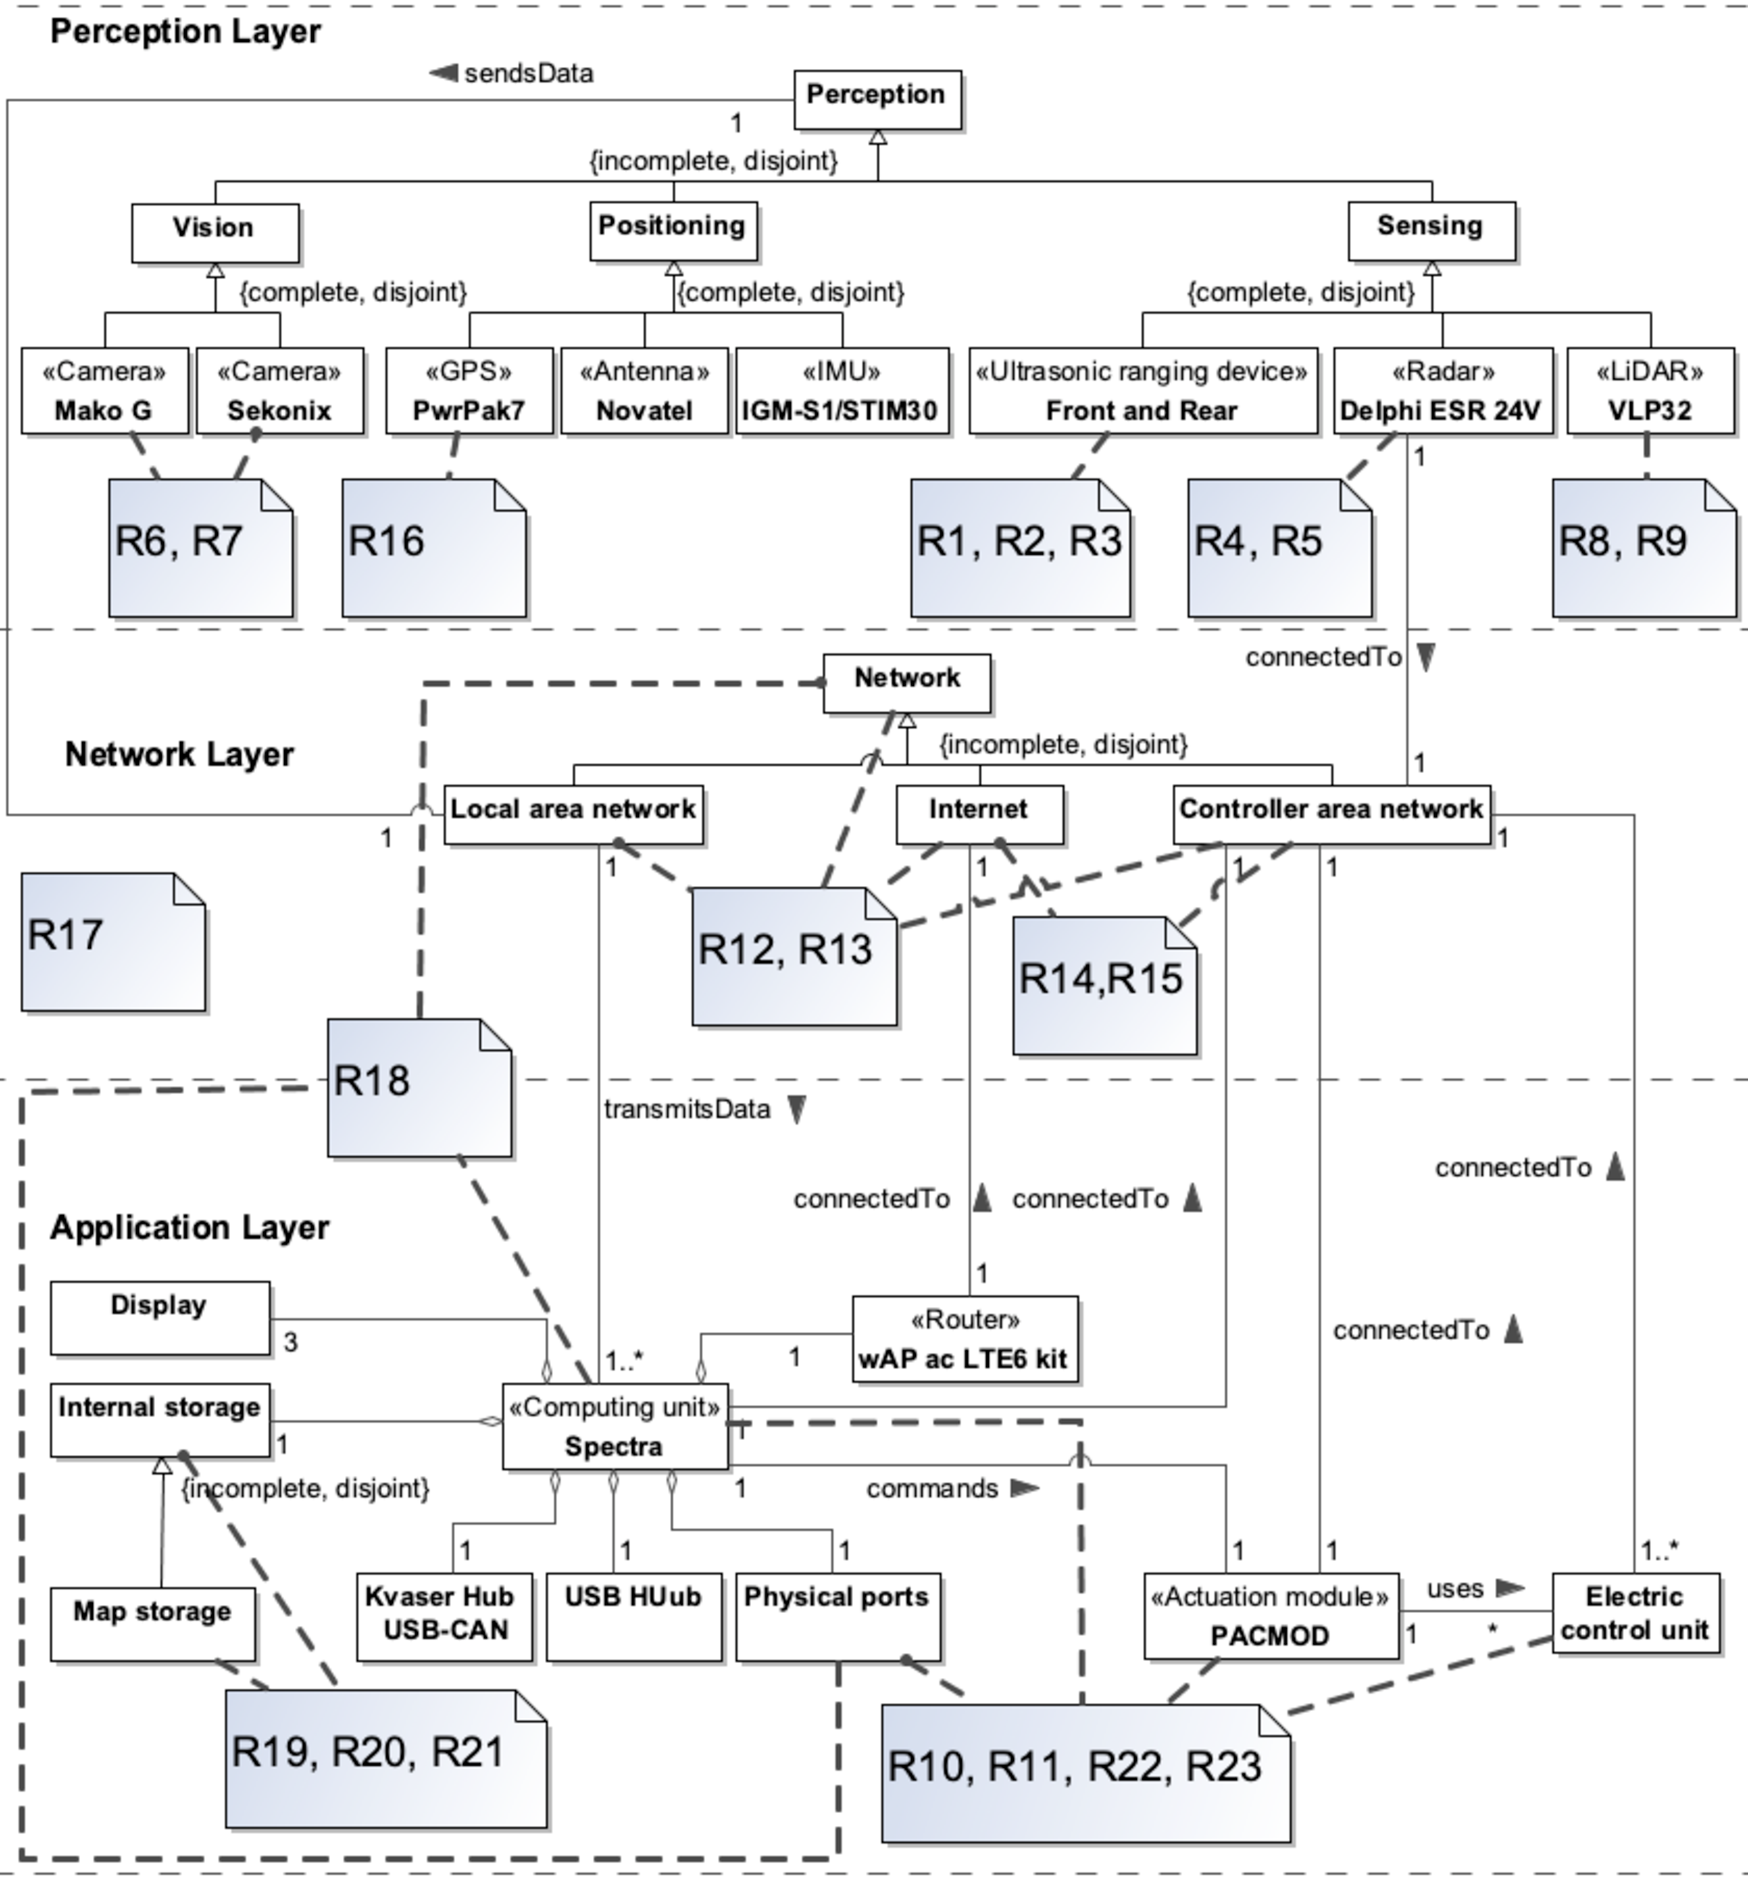
\includegraphics[width=0.8\linewidth]{AVassetsCase}
  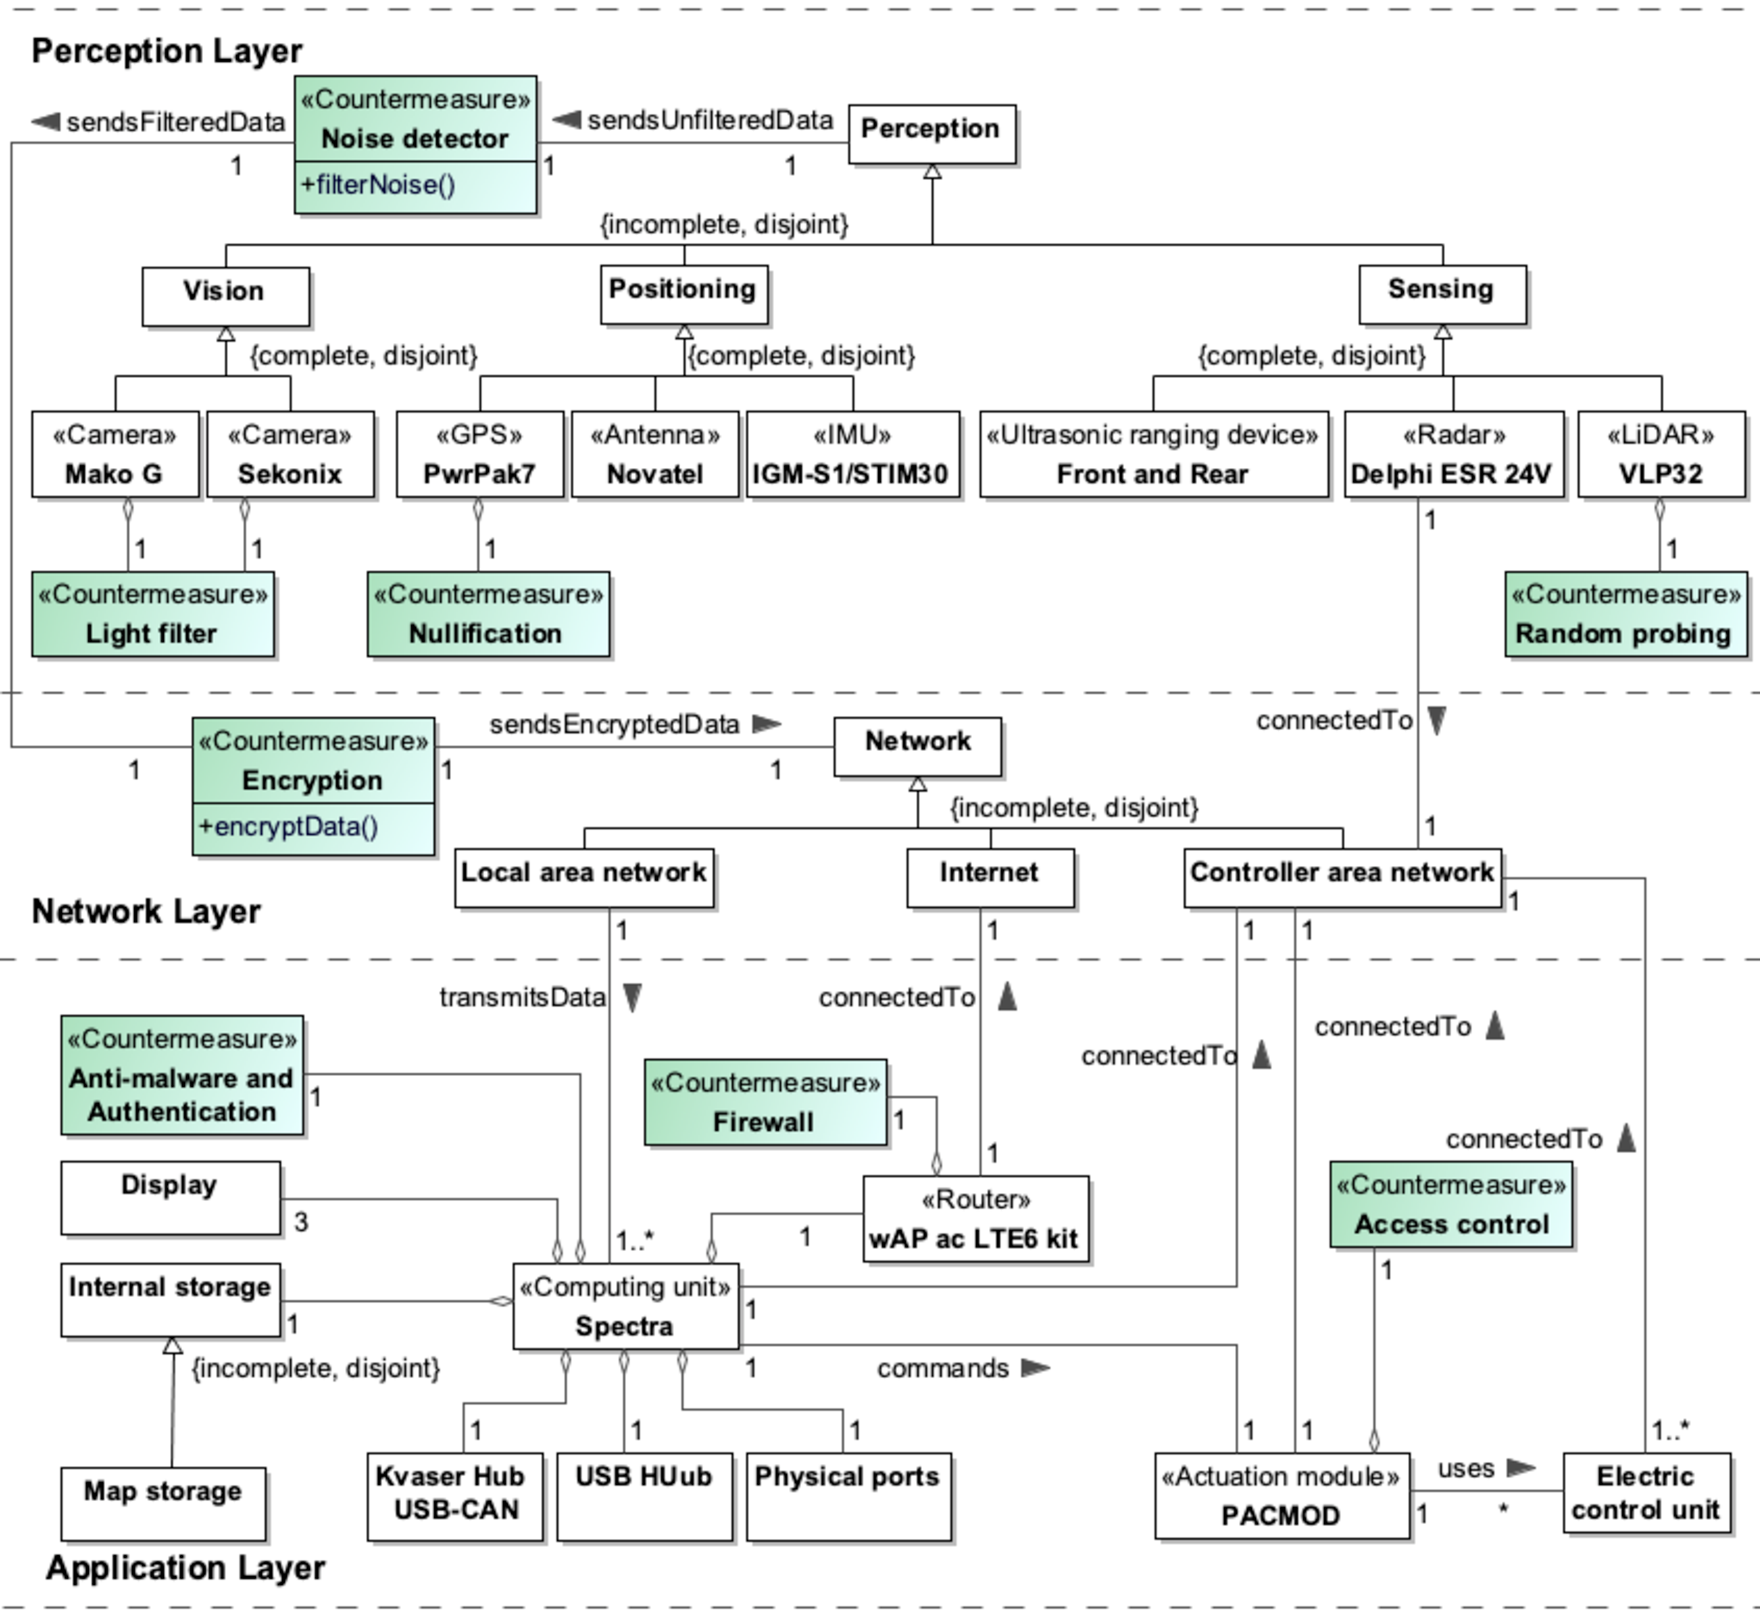
\includegraphics[width=0.8\linewidth]{caseCount}
   %\vspace{-5pt}
  \caption{Case analysis: Countermeasures} 
  \label{fig:Count}
  \vspace{-15pt}
\end{figure}

\hyperref[tab:mitigation-example]{Table~\ref{tab:mitigation-example}} illustrates the countermeasures to mitigate risk R6. Two controls are suggested: (\textit{i}) multiple sensors for redundancy check (i.e., \textit{image output (overlapping) with multiple cameras}) estimated with the low cost and (\textit{ii}) filter to remove harmful light -- with the \textit{high} cost. Full risk management documentation can then be compiled. \footnote{Detailed risk management documentation for the elicited security risks \url{https://git.io/Jfp55}}
%

\begin{table}[h!]
\caption{Case analysis: R6 mitigation}
\label{tab:mitigation-example}
\resizebox{\textwidth}{!}{%
\begin{tabular}{|l|l|l|l|l|l|l|l|l|l|}
\hline
\textbf{Risk Mitigation} & \multicolumn{9}{l|}{\textbf{R6: Blinding cameras}}                 \\ \hline
Choose   action to take. & Accept:        & \hspace{10mm} & Defer:        & \hspace{10mm} & Mitigate: & \hspace{5mm} x \hspace{5mm} & Transfer: & \multicolumn{2}{l|}{ \hspace{10mm} } \\ \hline
\multicolumn{10}{|l|}{\textbf{For the risk, what   actions and controls will be used:}}                      \\ \hline
Layer where applied      & \multicolumn{5}{l|}{Description of control or action}               & \multicolumn{4}{l|}{Estimated cost}   \\ \hline
Perception               & \multicolumn{5}{l|}{Image output (overlapping) with multiple cameras} & \multicolumn{4}{l|}{Low}              \\ \hline
Perception                 & \multicolumn{5}{l|}{Filter to remove harmful light} & \multicolumn{4}{l|}{High} \\ \hline
\end{tabular}%
}
 \vspace{-10pt}  
\end{table}


\section{Discussion (to be completed)}
\label{sec:disc}
In this study, we focused on the security risks to autonomous driving vehicles; however the scope only covered connected and autonomous components of the vehicle. We covered these autonomous assets, its data sources and security risks to the data, its interactions and the supporting system assets following the ISSRM method. We then provided an estimate for the security risk impacts using OCTAVE to produce outputs that can be consumed by the system stakeholders for the purpose of risk treatment prioritization and treatment decisions. In this section, we discuss the outcome of this research and how it answers our research questions.

%\subsection{Asset-related concepts}
The business assets of the AV systems covered data from multiple sources/~system assets necessary for the functionality of the AV. We also found that in IISs, the availability and manipulation of data and use of information is fundamental to its function. Although these business assets require protection following its security requirements, data categorization and analysis in AVs is also important for protection strategies to be developed. Robust and redundant data sources improve data collection, monitoring and analysis for autonomous driving vehicles and could potentially help in identifying anomalous inputs and behavior produced by cyber attacks. However, the availability and integrity of these data sources must be ensured to prevent compromise and the AV must create a trust boundary so that the it trusts sensors within a closer boundary more than external or unknown data sources (e.g., other vehicle or roadside system).


%\subsection{Risk-related concepts}
In this paper, the security risk estimation and management was done using a combination of the ISSRM and OCTAVE approaches.
From further analysis of the risks related to our case study, we discovered seemingly unconventional attacks to the AV that are not seen in literature. One of such is carrying out the blinding attack using mirrors to reflect sunlight. This could make the likelihood of \textbf{R7} \textit{high}, however, simply turning off auto exposure could be used as countermeasure.  Another is spoofing the \textit{LiDAR} with smoke, which increases the likelihood of a spoofing event as it is a low effort attack. However, possible countermeasure is to improve the obstacle detection algorithms. Lastly, an attack by changing the code used for implementing AV functions through the code repository was seen as a possibility where suggested countermeasures would include unit tests and manual checks to all code used by the AV \textit{ECU} implement AV functionalities.


Outlining  risk estimations enables proper risk treatment prioritisation and better return on investment (ROI) as regards treating prioritized security risks. Using OCTAVE, we were able to deduce the risk scores based on the relative scores of the threat impact on the affected assets and the threat likelihood, while providing a documented overview of the proposed risk to relevant stakeholders. 
In~\cite{Bailey2018}, the author has used the NIST risk assessment process~\cite{NIST}, combined it with some probabilistic method and applied the optimisation techniques to recommend the best countermeasures. Similarly, to~\cite{Bailey2018}, we have used the countermeasure cost estimation, but transformed the cost estimates to the qualitative values. This allows us to reduce the amount of collected data, but still contribute to decisions regarding the countermeasure selection. 
%The risk estimation values 




\section{Conclusion}
\label{sec:conc}
In this paper we have considered the security risks in the AV systems. More specifically we have performed the literature study, case analysis and discussed the outcomes of the outlined assets, security risks and their impact and countermeasures to mitigate these risks in AV. Our study indicates that business assets, characterised as data collected, communicated and manipulated at different layers of the AV architecture need to be protected for autonomous driving. The AV system assets including AV sensors, communication devices, computing unit and others also require protection. Thus, we have elicited, documented and estimated 24 security risks and recommended the countermeasures to mitigate them. 

Security risk management is an iterative activity. In this iteration we have considered security risks of AV components and its estimated risk value, useful for risk prioritization by AV stakeholders. The follow up activities needs to be carried on regarding vehicle. Similar to~\cite{Bailey2018}, there is also the need of establishing a quantitative security risk and countermeasure estimation approach. Although we have combined both the ISSRM and OCTAVE in this study, the nowadays growth and interest in the AV domain potentially require targeted approaches for the security risk management including different -- vehicle's information systems, vehicle and passenger interaction and other vehicle -- perspectives.



\bibliographystyle{splncs04}
\bibliography{references}


\end{document}
